\documentclass[12pt,a4paper,article,english,firamath]{nsi}
\pagestyle{empty}
\setfontfamily{\brettley}{Cursive standard}[Scale=1.5]
\begin{document}
\titre{Find your figure}
\classe{Euro 1\ere}
\maketitle

\subsection*{Description 5}
{\brettley 

Draw a line segment. Complete the figure with three other line segments to make a square. Then, draw two lines, each one
passing through the midpoints of two opposite sides of the square. Draw another line passing through two opposite
corners. Finally, draw a the circle passing through two corners of the square and its center.}\\[1em]

\begin{tikzpicture}
    \draw[lightgray](0,0)--(\linewidth,0);
\end{tikzpicture}


\subsection*{Figure 5}
\begin{center}
    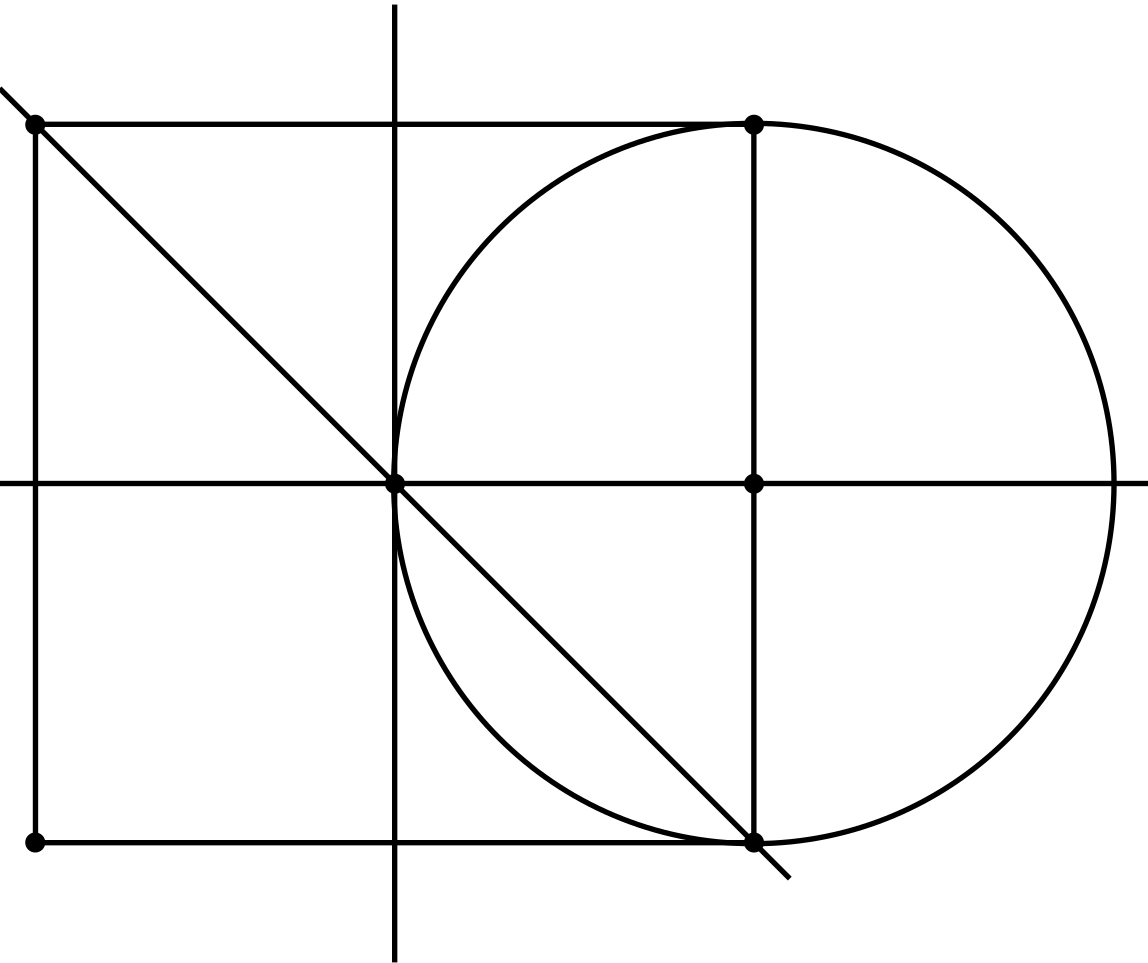
\includegraphics[height=12cm]{img/fig05.png}
\end{center}
\end{document}